\begin{figure}[htbp]
\centering
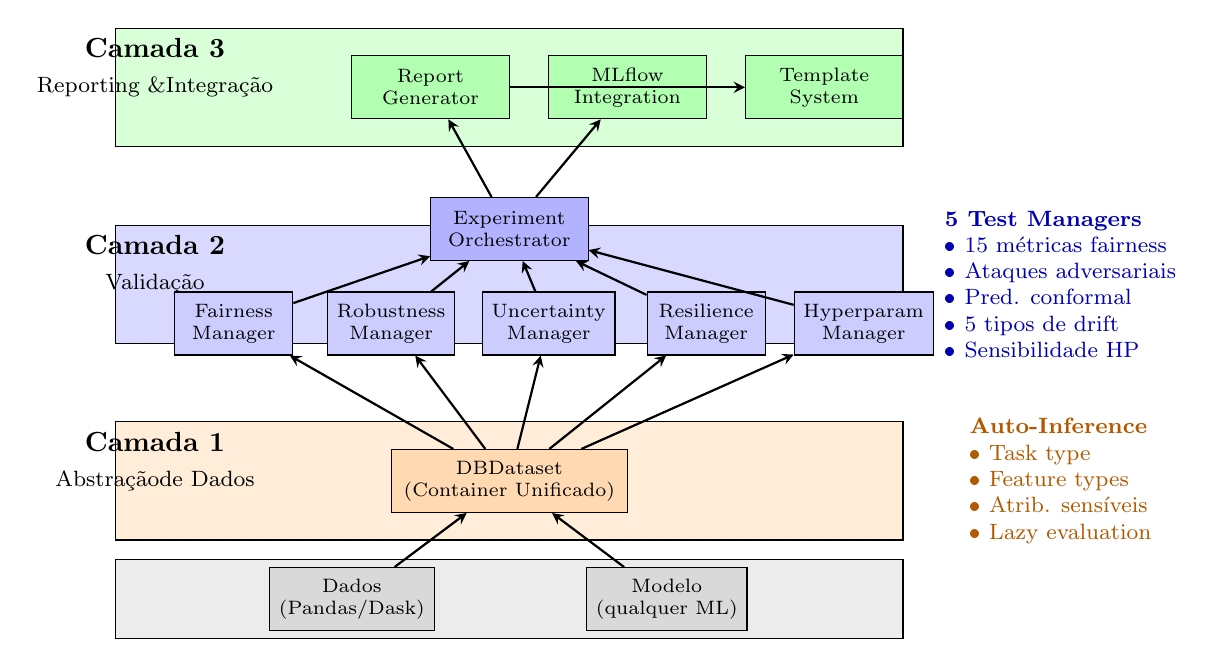
\begin{tikzpicture}[
    layer/.style={rectangle, draw, minimum width=10cm, minimum height=1.5cm, align=center, font=\small},
    component/.style={rectangle, draw, minimum width=2cm, minimum height=0.8cm, align=center, font=\scriptsize},
    arrow/.style={->, >=stealth, thick},
    label/.style={font=\footnotesize}
]

% Camada 3: Reporting e Integração
\node[layer, fill=green!15] (layer3) at (0,0) {};
\node[font=\bfseries] at (-4.5,0.5) {Camada 3};
\node[label] at (-4.5,0) {Reporting \&\\Integração};

\node[component, fill=green!30] (report) at (-1,0) {Report\\Generator};
\node[component, fill=green!30] (mlflow) at (1.5,0) {MLflow\\Integration};
\node[component, fill=green!30] (templates) at (4,0) {Template\\System};

% Camada 2: Validação
\node[layer, fill=blue!15] (layer2) at (0,-2.5) {};
\node[font=\bfseries] at (-4.5,-2) {Camada 2};
\node[label] at (-4.5,-2.5) {Validação};

\node[component, fill=blue!30] (experiment) at (0,-1.8) {Experiment\\Orchestrator};

\node[component, fill=blue!20, minimum width=1.5cm] (fairness) at (-3.5,-3) {Fairness\\Manager};
\node[component, fill=blue!20, minimum width=1.5cm] (robust) at (-1.5,-3) {Robustness\\Manager};
\node[component, fill=blue!20, minimum width=1.5cm] (uncertain) at (0.5,-3) {Uncertainty\\Manager};
\node[component, fill=blue!20, minimum width=1.5cm] (resilience) at (2.5,-3) {Resilience\\Manager};
\node[component, fill=blue!20, minimum width=1.5cm] (hyperparam) at (4.5,-3) {Hyperparam\\Manager};

% Camada 1: Abstração de Dados
\node[layer, fill=orange!15] (layer1) at (0,-5) {};
\node[font=\bfseries] at (-4.5,-4.5) {Camada 1};
\node[label] at (-4.5,-5) {Abstração\\de Dados};

\node[component, fill=orange!30, minimum width=3cm] (dbdataset) at (0,-5) {DBDataset\\(Container Unificado)};

% Camada 0: Dados e Modelos
\node[layer, fill=gray!15, minimum height=1cm] (layer0) at (0,-6.5) {};
\node[component, fill=gray!30] (data) at (-2,-6.5) {Dados\\(Pandas/Dask)};
\node[component, fill=gray!30] (model) at (2,-6.5) {Modelo\\(qualquer ML)};

% Setas entre camadas
\draw[arrow] (data) -- (dbdataset);
\draw[arrow] (model) -- (dbdataset);

\draw[arrow] (dbdataset) -- (fairness);
\draw[arrow] (dbdataset) -- (robust);
\draw[arrow] (dbdataset) -- (uncertain);
\draw[arrow] (dbdataset) -- (resilience);
\draw[arrow] (dbdataset) -- (hyperparam);

\draw[arrow] (fairness) -- (experiment);
\draw[arrow] (robust) -- (experiment);
\draw[arrow] (uncertain) -- (experiment);
\draw[arrow] (resilience) -- (experiment);
\draw[arrow] (hyperparam) -- (experiment);

\draw[arrow] (experiment) -- (report);
\draw[arrow] (experiment) -- (mlflow);
\draw[arrow] (report) -- (templates);

% Anotações laterais
\node[label, text=blue!70!black, align=left] at (7,-2.5) {
\textbf{5 Test Managers}\\
\textbullet~15 métricas fairness\\
\textbullet~Ataques adversariais\\
\textbullet~Pred. conformal\\
\textbullet~5 tipos de drift\\
\textbullet~Sensibilidade HP
};

\node[label, text=orange!70!black, align=left] at (7,-5) {
\textbf{Auto-Inference}\\
\textbullet~Task type\\
\textbullet~Feature types\\
\textbullet~Atrib. sensíveis\\
\textbullet~Lazy evaluation
};

\end{tikzpicture}
\caption{Arquitetura em três camadas do DeepBridge. Camada 1 (DBDataset) provê abstração unificada de dados/modelos. Camada 2 (Experiment + Test Managers) orquestra validação multi-dimensional. Camada 3 (Reporting) gera relatórios audit-ready e integra com MLOps.}
\label{fig:architecture}
\end{figure}
